\setcounter{framenumber}{0}
%28

\begin{frame}
  \titlepage
\end{frame}

\begin{frame}{Learning Goals}
By the end of this lecture, students should be able to:
\begin{itemize}
    \item explain probability as a mathematical language for uncertainty;
    \item identify a sample space for a random experiment;
    \item distinguish between outcomes and events;
    \item translate basic probability statements into set notation;
    \item use unions, intersections, complements, and De Morgan's laws;
\end{itemize}
\end{frame}

\begin{frame}{Why Study Probability?}
\begin{keybox}{Central idea}
Probability is the logic of uncertainty.
\end{keybox}

\vspace{0.25cm}

Probability provides tools for:
\begin{itemize}
    \item modeling randomness and uncertainty;
    \item understanding variation and separating signal from noise (blood pressure)
    \item making principled predictions and decisions;
    \item quantifying risk;
    \item avoiding misleading or incomplete intuition.
\end{itemize}
\end{frame}




\begin{frame}{Three Habits for This Course}
\begin{enumerate}
    \item \textbf{Biohazards.}  
    Study common mistakes so that invalid reasoning becomes easier to detect.

    \item \textbf{Sanity checks.}  
    After solving a problem, check whether the answer makes sense in simple or extreme cases.

    \item \textbf{Conceptual clarity.}  
    Make sure the sample space, events, and assumptions are clearly specified before assigning probabilities.
\end{enumerate}

\vspace{0.3cm}

\begin{keybox}{Guiding principle}
Good probability reasoning starts with precise modeling, not just calculations.
\end{keybox}
\end{frame}

\lecturepart{Sample Spaces and Events}

\begin{frame}{Random Experiments}
A \textbf{random experiment} is a process whose outcome is uncertain before it is performed.

\vspace{0.3cm}

Examples:
\begin{itemize}
    \item flipping a coin;
    \item rolling a die;
    \item drawing a card from a shuffled deck;
    \item recording tomorrow's temperature;
    \item selecting a student from the class;
    \item measuring the lifetime of a machine component.
\end{itemize}

\vspace{0.25cm}

\begin{keybox}{Important}
Before assigning probabilities, the possible outcomes must be clearly specified.
\end{keybox}
\end{frame}

\begin{frame}{Definition: Sample Space and Event}
\begin{keybox}{Definition}
The \textbf{sample space} $\Sample$ of an experiment is the set of all possible outcomes.

An \textbf{event} $A$ is a subset of the sample space:
\[
A \subseteq \Sample.
\]

The event $A$ occurs if the actual outcome belongs to $A$:
\[
\actual \in A.
\]
\end{keybox}

\vspace{0.25cm}

\begin{itemize}
    \item An \textbf{outcome} is a single element of $\Sample$.
    \item An \textbf{event} is a collection of outcomes.
    \item The sample space is the universal set for the experiment.
    \item Some textbooks use $\Omega$ instead of $\Sample$, and $\omega $ instead of $s$
\end{itemize}
\end{frame}

\begin{frame}{Pebble World Picture}
When the sample space is finite, imagine each possible outcome as a pebble.

\[
\Sample = \{\text{all pebbles}\}
\]

\begin{center}
\begin{tikzpicture}[scale=0.82]
    \draw[rounded corners, thick] (-3.4,-1.65) rectangle (3.4,1.65);
    \node at (3.0,1.30) {$\Sample$};

    \foreach \x/\y in {-2.8/0.9,-2.1/1.1,-1.3/0.75,-0.3/0.95,0.8/0.9,2.1/0.95,
                       -2.4/0.0,-1.5/0.05,-0.5/0.10,0.6/0.0,1.7/0.1,2.6/0.0,
                       -2.7/-0.8,-1.8/-0.95,-0.7/-0.75,0.5/-0.85,1.6/-0.75,2.5/-0.85}
        \fill[UWGray] (\x,\y) circle (2.5pt);

    % A is now fully inside the sample space
    \draw[UWPurple, thick] (-2.25,-0.25) ellipse (0.95 and 1.05);
    \node[UWPurple] at (-2.75,1.25) {$A$};

    \draw[UWGold!80!black, thick] (0.55,-0.05) ellipse (1.55 and 1.05);
    \node[UWGold!80!black] at (0.15,1.25) {$B$};
\end{tikzpicture}
\end{center}

\begin{itemize}
    \item Each pebble represents an outcome.
    \item An event is a set of pebbles.
    \item Performing the experiment selects one pebble.
    \item The event occurs if the selected pebble lies in the event.
\end{itemize}
\end{frame}

\begin{frame}{Types of Sample Spaces}
Sample spaces can be:

\begin{enumerate}
    \item \textbf{Finite}
    \[
    \Sample = \{1,2,3,4,5,6\}
    \]
    for rolling one die.

    \item \textbf{Countably infinite}
    \[
    \Sample = \{1,2,3,\dots\}
    \]
    for the number of tosses until the first head.

    \item \textbf{Uncountable}
    \[
    \Sample = [0,\infty)
    \]
    for the lifetime of a machine component.
\end{enumerate}

\vspace{0.15cm}

\begin{keybox}{For now}
Many early examples use finite sample spaces, where outcomes can be counted.
\end{keybox}
\end{frame}

\lecturepart{Set Operations for Events}

\begin{frame}{Union, Intersection, Complement}
Let $A,B \subseteq \Sample$ be events.

\begin{center}
\begin{tabular}{lll}
\toprule
Set operation & Notation & Meaning \\
\midrule
Union & $A \cup B$ & $A$ or $B$ occurs, possibly both \\
Intersection & $A \cap B$ & both $A$ and $B$ occur \\
Complement & $A^c $ (or $A^\prime$) & $A$ does not occur \\
\bottomrule
\end{tabular}
\end{center}

\vspace{0.25cm}

\begin{keybox}{Notation}
Some textbooks write $A'$ for the complement of $A$.  
In this course, we write $A^c$ instead, because prime notation is also used for differentiation, such as $f'(x)$.
\end{keybox}
\end{frame}
\begin{frame}{Venn Diagrams for Basic Set Operations}

\begin{center}
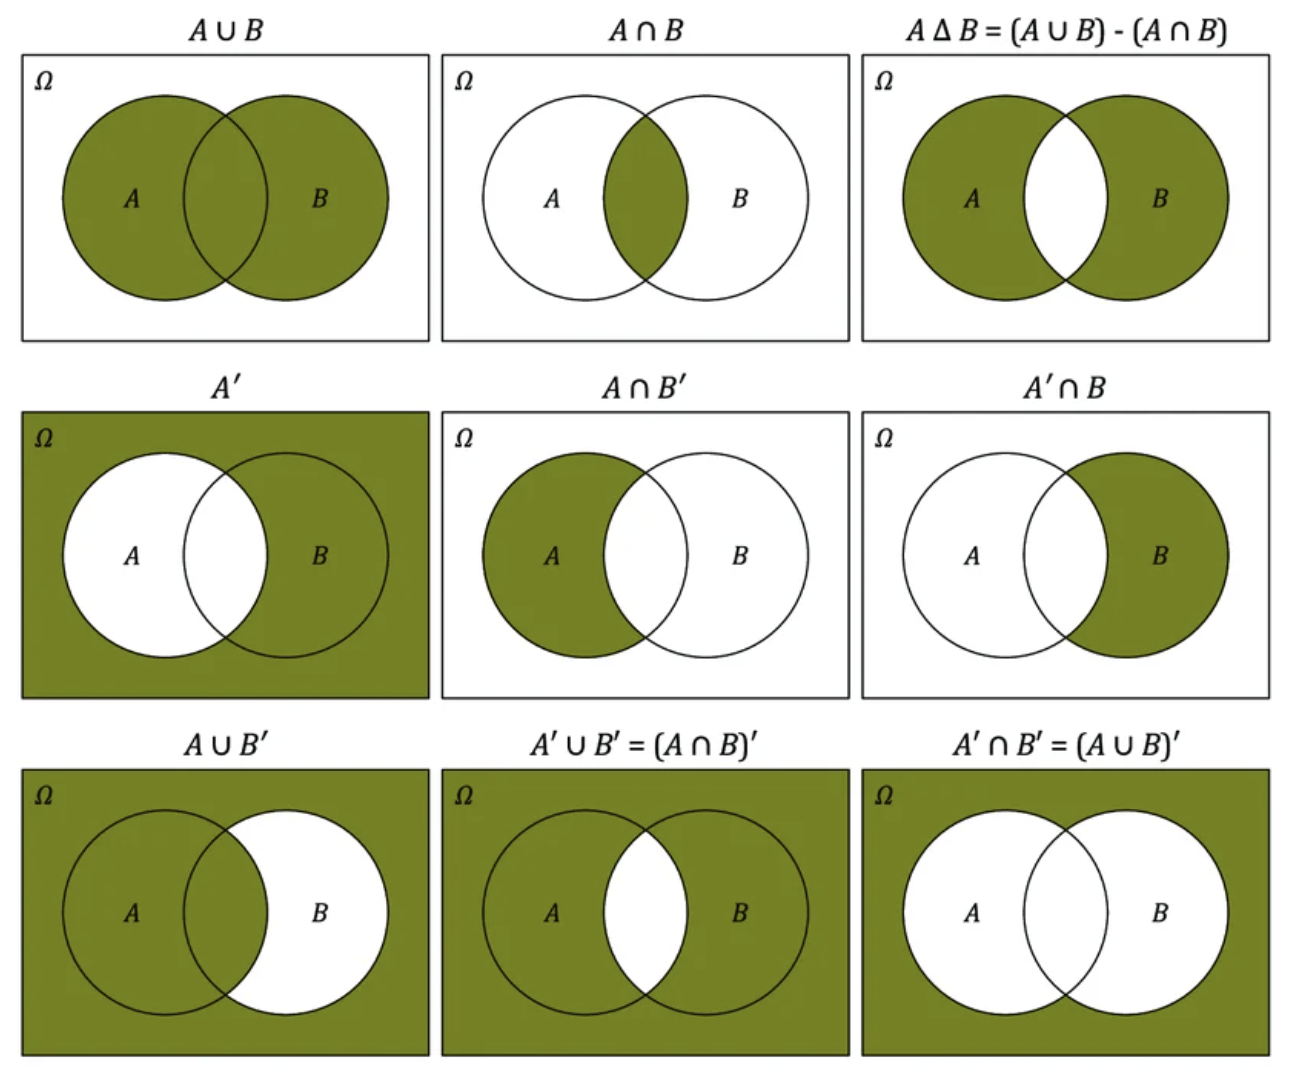
\includegraphics[width=0.48\textwidth]{assets/figures/van.png}
\end{center}

\vspace{-0.3cm}

\begin{center}
{\scriptsize The green area represents the formula above each diagram. Source: 
\href{https://www.researchgate.net/figure/A-Venn-diagram-of-unions-and-intersections-for-two-sets-A-and-B-and-their-complements_fig1_332453167}{ResearchGate Figure}}
\end{center}

\vspace{-0.1cm}

\begin{center}
{\small Here $\Omega$ represent the sample space ($\Sample$) and $A^\prime$ represent complement of $A$, i.e., $A^c$ .}
\end{center}

\end{frame}

\begin{frame}{Example: Ten Coin Flips}
Suppose a coin is flipped $10$ times.

\[
\Sample = \{(s_1,\dots,s_{10}) : s_j \in \{H,T\},\ 1 \le j \le 10\}.
\]

There are
\[
|\Sample| = 2^{10}
\]
possible outcomes.

Let $A_j$ be the event that the $j$th flip is heads:
\[
A_j = \{(s_1,\dots,s_{10}) \in \Sample : s_j = H\}.
\]

\[
\text{At least one head}
= \bigcup_{j=1}^{10} A_j.
\]

\[
\text{All flips are heads}
= \bigcap_{j=1}^{10} A_j.
\]

\[
\text{At least two consecutive heads}
= \bigcup_{j=1}^{9} (A_j \cap A_{j+1}).
\]
\end{frame}

\begin{frame}{The Empty Set}
The \textbf{empty set} is the set with no elements. It is denoted by
\[
\emptyset.
\]

\vspace{0.2cm}

Important facts:
\begin{itemize}
    \item $\emptyset$ means ``nothing occurred'' or ``no outcome is included.''
    \item For every set $A$,
    \[
    A \cap \emptyset = \emptyset.
    \]
    \item For every set $A$,
    \[
    A \cup \emptyset = A.
    \]
    \item The empty set is a subset of every set:
    \[
    \emptyset \subseteq A.
    \]
\end{itemize}
\end{frame}

\begin{frame}{Important Set Notation Clarifications}
\begin{keybox}{Singletons versus elements}
The object $2$ is not the same as the set $\{2\}$.

\[
2 \neq \{2\}.
\]

The set $\{2\}$ is the set whose only element is $2$.
\end{keybox}

\vspace{0.25cm}

Similarly,
\[
\emptyset \neq \{\emptyset\}.
\]

\begin{itemize}
    \item $\emptyset$ has no elements.
    \item $\{\emptyset\}$ has one element, namely $\emptyset$.
\end{itemize}

\vspace{0.2cm}

So:
\[
|\emptyset| = 0,
\qquad
|\{\emptyset\}| = 1.
\]
\end{frame}

\begin{frame}{Events as Sets: $A$ versus $\{A\}$}
Suppose $A$ is an event. Then $A$ is already a set of outcomes.

For example, if
\[
\Sample = \{1,2,3,4,5,6\},
\qquad
A = \{2,4,6\},
\]
then $A$ is the event that the die roll is even.

\vspace{0.25cm}

But
\[
\{A\} = \big\{\{2,4,6\}\big\}
\]
is a set whose single element is the set $A$.

\vspace{0.25cm}

\begin{keybox}{Common mistake}
Usually, $A \subseteq \Sample$, but $\{A\}$ is not a subset of $\Sample$ unless $A$ itself is an outcome.
\end{keybox}
\end{frame}

\begin{frame}{De Morgan's Laws}
For events $A,B \subseteq \Sample$,

\[
(A \cup B)^c = A^c \cap B^c,
\]

\[
(A \cap B)^c = A^c \cup B^c.
\]

\vspace{0.3cm}

Interpretation:

\begin{itemize}
    \item Not having at least one of $A$ or $B$ means having neither.
    \item Not having both $A$ and $B$ means at least one fails to occur.
\end{itemize}

\vspace{0.25cm}

\begin{livebox}{Optional live verification}
Draw a Venn diagram and shade both sides of each identity.
\end{livebox}
\end{frame}

\begin{frame}{Union and Intersection of Many Events}
Let $A_1,A_2,\dots,A_n \subseteq \Sample$.

The union is the event that \textbf{at least one} of the events occurs:
\[
\bigcup_{i=1}^n A_i
=
\{s \in \Sample : s \in A_i \text{ for at least one } i \in \{1,\dots,n\}\}.
\]

The intersection is the event that \textbf{all} of the events occur:
\[
\bigcap_{i=1}^n A_i
=
\{s \in \Sample : s \in A_i \text{ for every } i \in \{1,\dots,n\}\}.
\]

\vspace{0.25cm}

For infinitely many events $A_1,A_2,\dots$:
\[
\bigcup_{i=1}^{\infty} A_i
=
\{s \in \Sample : s \in A_i \text{ for at least one } i\}, \quad \quad \bigcap_{i=1}^{\infty} A_i
=
\{s \in \Sample : s \in A_i \text{ for every } i\}.
\]

Question: What does demorgan law generalize to, for a union of (infinitely many) events?
\end{frame}

\begin{frame}{Example: Drawing One Card}
Draw one card from a standard $52$-card deck.

Define:
\[
A = \{\text{card is an ace}\},
\qquad
B = \{\text{card has a black suit}\},
\]
\[
D = \{\text{card is a diamond}\},
\qquad
H = \{\text{card is a heart}\}.
\]

Then:
\[
A \cap H = \{\text{Ace of Hearts}\},
\]

\[
A \cap B = \{\text{Ace of Spades, Ace of Clubs}\},
\]

\[
D \cap H = \emptyset,
\]
because no card can be both a diamond and a heart.

\[
A \cup D \cup H = \{\text{card is red or an ace}\}.
\]
\end{frame}

\begin{frame}{Card Example: Complements}
Using De Morgan's laws,

\[
(A \cup B)^c = A^c \cap B^c.
\]

So:

\[
(A \cup B)^c
=
\{\text{card is not an ace and not black}\}.
\]

Equivalently,

\[
(A \cup B)^c
=
\{\text{card is a red non-ace}\}.
\]

Also,

\[
(D \cup H)^c = D^c \cap H^c = B.
\]

\begin{keybox}{Lesson}
The same event can often be expressed in more than one way. Some expressions are much easier to use than others.
\end{keybox}
\end{frame}

\begin{frame}{A Subtle Point: Is the Sample Space Correct?}
In the card example, the sample space is the set of all $52$ standard cards.

\vspace{0.3cm}

If the drawn card is a joker, then the issue is not probability calculation.

\vspace{0.2cm}

The issue is:
\[
\textbf{the sample space was wrong.}
\]

\vspace{0.3cm}

\begin{keybox}{Rule}
The sample space must contain every outcome that can actually occur.
\end{keybox}
\end{frame}

\lecturepart{English $\longleftrightarrow$ Set Notation}

\begin{frame}{Dictionary: Events and Occurrences}
Let $\actual$ be the actual outcome.

\begin{center}
\begin{tabular}{ll}
\toprule
English statement & Set notation \\
\midrule
sample space & $\Sample$ \\
$s$ is a possible outcome & $s \in \Sample$ \\
$A$ is an event & $A \subseteq \Sample$ \\
$A$ occurred & $\actual \in A$ \\
something must happen & $\actual \in \Sample$ \\
\bottomrule
\end{tabular}
\end{center}

\vspace{0.3cm}

\begin{keybox}{Conceptual point}
Events are not numbers. Events are sets. Probability will later assign numbers to events.
\end{keybox}
\end{frame}

\begin{frame}{Dictionary: New Events from Old Events}
\begin{center}
\begin{tabular}{ll}
\toprule
English statement & Set notation \\
\midrule
$A$ or $B$ & $A \cup B$ \\
$A$ and $B$ & $A \cap B$ \\
not $A$ & $A^c$ \\
$A$ or $B$, but not both & $(A \cap B^c) \cup (A^c \cap B)$ \\
at least one of $A_1,\dots,A_n$ & $\displaystyle \bigcup_{j=1}^n A_j$ \\
all of $A_1,\dots,A_n$ & $\displaystyle \bigcap_{j=1}^n A_j$ \\
\bottomrule
\end{tabular}
\end{center}

\vspace{0.25cm}

\begin{keybox}{Notation reminder}
We write $A^c$ for complement, not $A'$.
\end{keybox}
\end{frame}

\begin{frame}{Dictionary: Relationships Between Events}
\begin{center}
\begin{tabular}{ll}
\toprule
English statement & Set notation \\
\midrule
$A$ implies $B$ & $A \subseteq B$ \\
$A$ and $B$ are mutually exclusive & $A \cap B = \emptyset$ \\
$A_1,\dots,A_n$ form a partition of $\Sample$ &
$\begin{array}{l}
A_1 \cup \cdots \cup A_n = \Sample,\\
A_i \cap A_j = \emptyset \text{ for } i \ne j
\end{array}$ \\
\bottomrule
\end{tabular}
\end{center}

\vspace{0.3cm}

\begin{keybox}{Partition}
A partition divides the sample space into non-overlapping pieces that together cover all possible outcomes.
\end{keybox}
\end{frame}

\begin{frame}{Mini-Exercise: Translate to Set Notation}
Let $A_j$ be the event that the $j$th coin flip is heads.

Translate each statement:

\begin{enumerate}
    \item The first flip is tails.
    \item The first two flips are heads.
    \item At least one of the first three flips is heads.
    \item None of the first three flips is heads.
    \item Exactly one of the first two flips is heads.
\end{enumerate}

\vspace{0.25cm}

\begin{livebox}{Optional answers}
\[
A_1^c,\qquad
A_1 \cap A_2,\qquad
A_1 \cup A_2 \cup A_3,
\]
\[
(A_1 \cup A_2 \cup A_3)^c
=
A_1^c \cap A_2^c \cap A_3^c,
\]
\[
(A_1 \cap A_2^c) \cup (A_1^c \cap A_2).
\]
\end{livebox}
\end{frame}

\begin{frame}{Common Mistake}
\begin{keybox}{Biohazard}
Do not confuse an outcome with an event.
\end{keybox}

\vspace{0.3cm}

For one die roll:
\[
\Sample = \{1,2,3,4,5,6\}.
\]

The number $4$ is an outcome.

The event ``the roll is even'' is the set
\[
E = \{2,4,6\}.
\]

So:
\[
4 \in \Sample,
\qquad
E \subseteq \Sample.
\]

\begin{livebox}{Emphasis}
Writing $E \in \Sample$ is wrong here because $E$ is a set of outcomes, not a single outcome.
\end{livebox}
\end{frame}

\begin{frame}{Summary}
\begin{itemize}
    \item Probability begins with a random experiment, and then, a clearly specified sample space $\Sample$.
    \item Outcomes are elements of $\Sample$ (i.e., $s\in S$).
    \item Events are subsets of $\Sample$ (i.e., $A\subseteq S$).
    \item Set operations:  allow us to build complicated events from simpler events.
    \item De Morgan's laws:  essential tools for rewriting complements.
    \item Choosing the correct sample space is part of the modeling process.
\end{itemize}

\vspace{0.3cm}

\begin{keybox}{Next lecture}
Naive probability: when outcomes are equally likely, probability becomes counting.
\end{keybox}
\end{frame}